\section{Membuat Halaman Chart}
Pada aplikasi ini kita akan membuat chart, yaitu chart tentang jurusan yang terbanyak terdata dari tabel jurusan dan mahasiswa.
\begin{itemize}
    \item[1] pertama siapkan terlebih dahulu query View CHART\_JURUSAN seperti berikut :
        \begin{lstlisting}
CREATE OR REPLACE FORCE EDITIONABLE VIEW  "CHART_JURUSAN" ("JURUSAN", "JUMLAH") AS 
  SELECT nama_jurusan, COUNT(nama_jurusan) AS jumlah FROM data_mhs GROUP BY nama_jurusan;        
        \end{lstlisting}
    \item[2] lalu ke halaman aplikasi anda kembali, lalu pilih create page
    \item[3] Pilih Chart, lihat pada Gambar 9.1.
    \begin{figure}
        \centering
        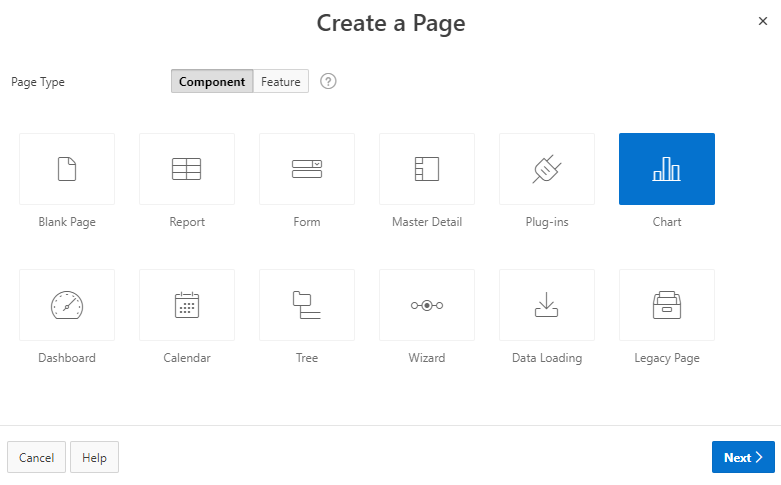
\includegraphics[scale=0.5]{figures/chart/chart1.png}
        \caption{\textit{Memilih Chart}}
        \label{Pilih Chart}
    \end{figure}

    \item[4]Pilih chart sesuai kesukaan anda , saya memilih BAR, lihat pada Gambar 9.2.
    \begin{figure}
        \centering
        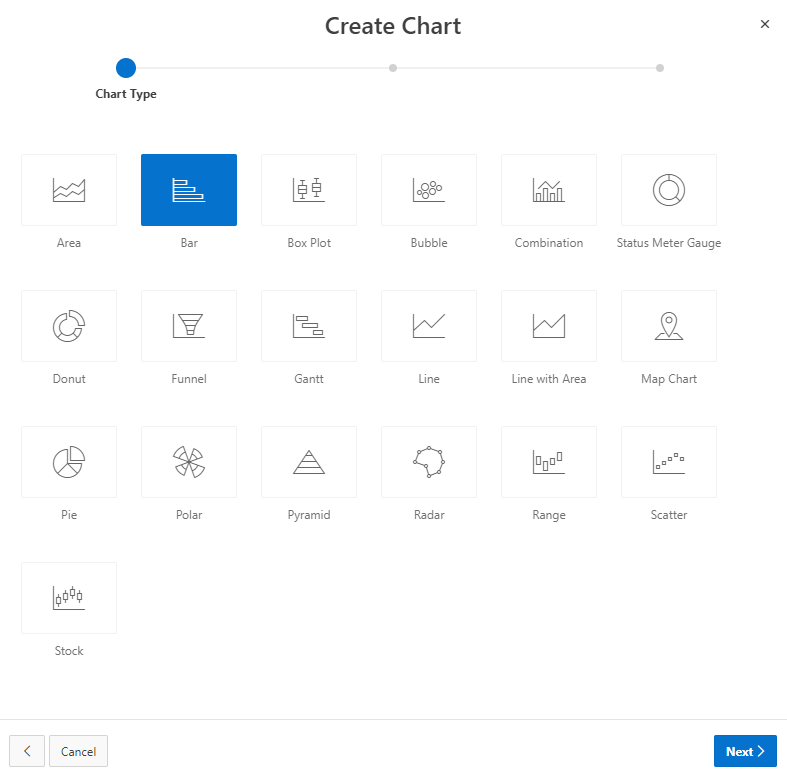
\includegraphics[scale=0.5]{figures/chart/chart2.png}
        \caption{\textit{Memilih Bar}}
        \label{Pilih Bar}
    \end{figure}

    \item[5]Pada form selanjutnya anda akan melihat Page Number,Name,dan Module, ikuti intruksi warna, lihat pada Gambar 9.3.
    \begin{figure}
        \centering
        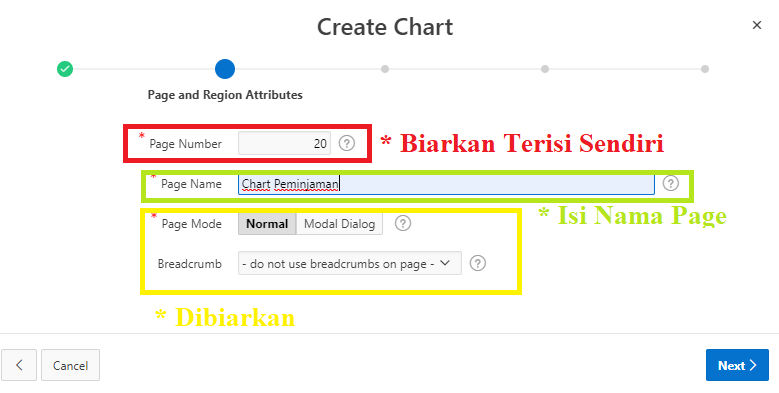
\includegraphics[scale=0.5]{figures/chart/chart3.png}
        \caption{\textit{Page Region And Attributes}}
        \label{Page Region And Attributes}
    \end{figure}
    \item[6]Pada form selanjutnya adalah menu navigasi, halaman anda akan disimpan pada navigasi apa, berikut petunjuk intruksi warna, lihat pada Gambar 9.4.
    \begin{figure}
        \centering
        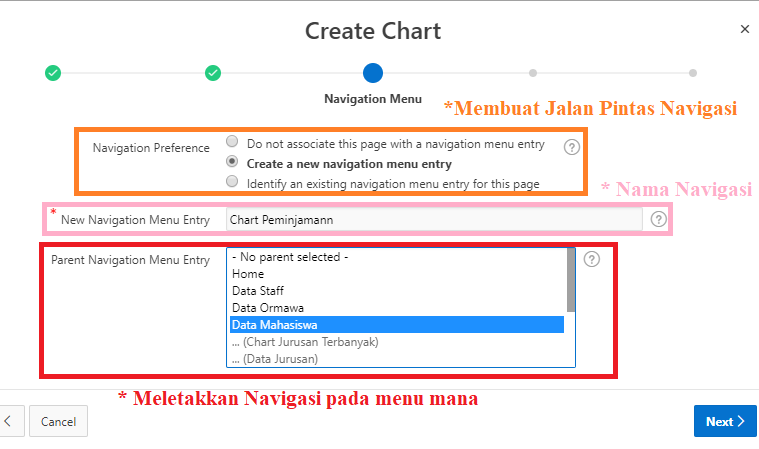
\includegraphics[scale=0.5]{figures/chart/chart4.png}
        \caption{\textit{Menu Navigasi}}
        \label{Menu Navigasi}
    \end{figure}
    \item[7]Pada form selanjutnya yaitu mengetahui source dari tabel apa, disini kita pilih view yang telah dibuat tadi yaitu CHART\_JURUSAN, ikuti intruksi warna, lihat pada Gambar 9.5.
    \begin{figure}
        \centering
        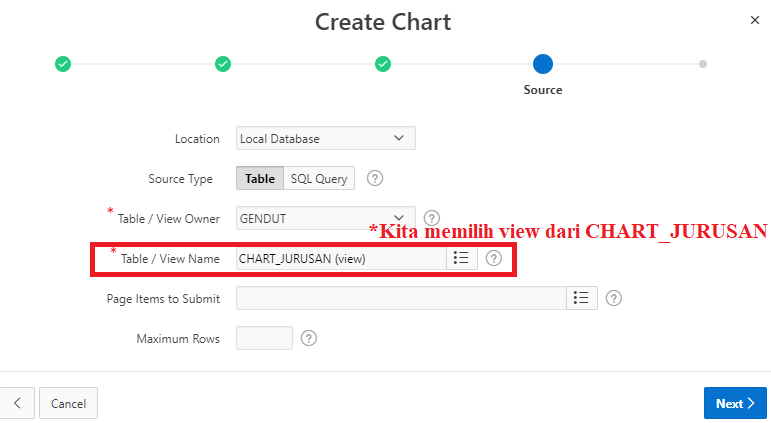
\includegraphics[scale=0.5]{figures/chart/chart5.png}
        \caption{\textit{Source}}
        \label{Source}
    \end{figure}
    \item[8]Pada form selanjutnya adalah mapping kolom untuk mengetahui label dan value yang akan ditampilkan pada chart, ikuti intruksi warna, lihat pada gambar 9.6.
    \begin{figure}
        \centering
        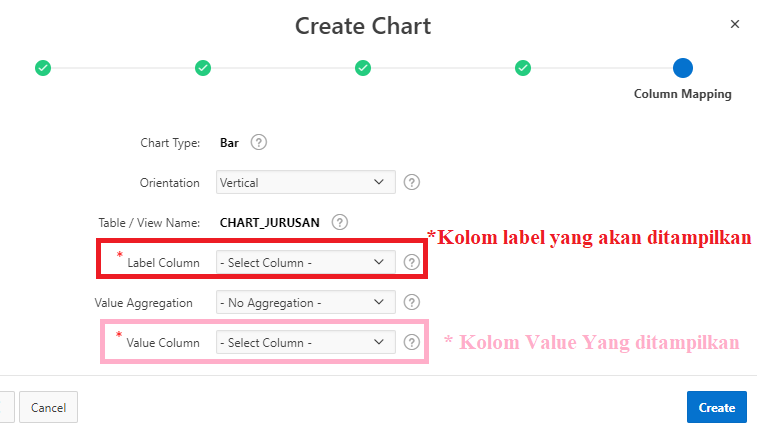
\includegraphics[scale=0.5]{figures/chart/chart6.png}
        \caption{\textit{Column Mapping}}
        \label{Column Mapping}
    \end{figure}
    \item[9]Anda bisa langsung mengecek dengan RUN aplikasi anda seperti Gambar 9.7.
    \begin{figure}
        \centering
        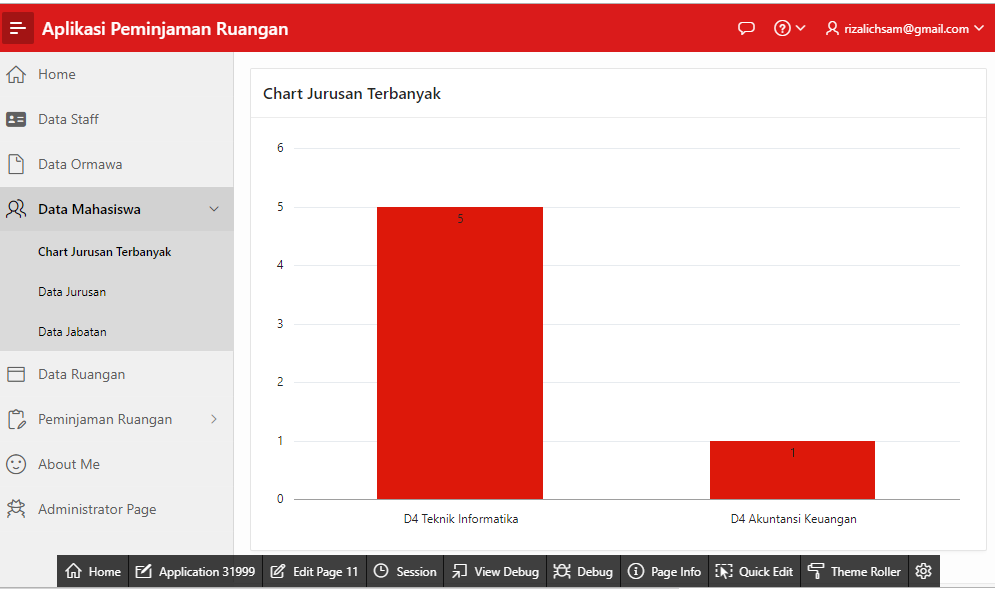
\includegraphics[scale=0.4]{figures/chart/chart7.png}
        \caption{\textit{Tampilan Chart}}
        \label{Tampilan Chart}
    \end{figure}
\end{itemize}
\section{Membuat Halaman CALENDAR}
Pada sesi ini kita akan membuat halaman DATE , yaitu menampilkan data dari database dengan berdasarkan tanggal peminjaman, ikuti langkah berikut.
\begin{itemize}
    \item[1]Pilih Calendar, lihat pada Gambar 9.8.
    \begin{figure}
        \centering
        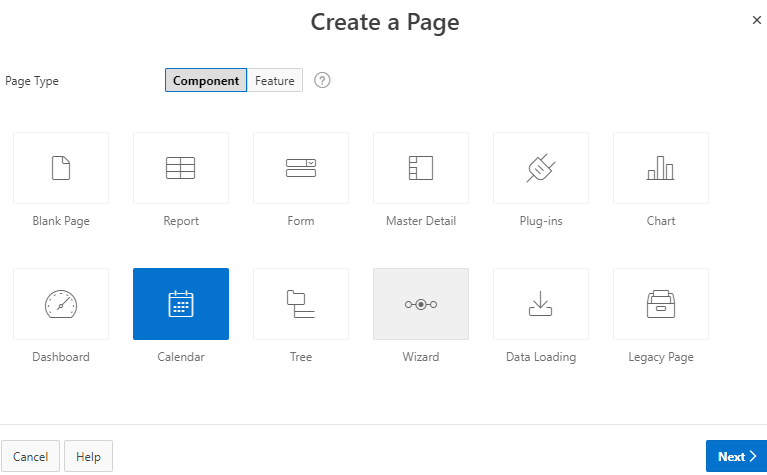
\includegraphics[scale=0.4]{figures/date/date1.png}
        \caption{\textit{Pilih Calendar}}
        \label{Pilih Calendar}
    \end{figure}
    \item[2]Membuat Page Name, ikuti intruksi warna, lihat pada Gambar 9.9.
    \begin{figure}
        \centering
        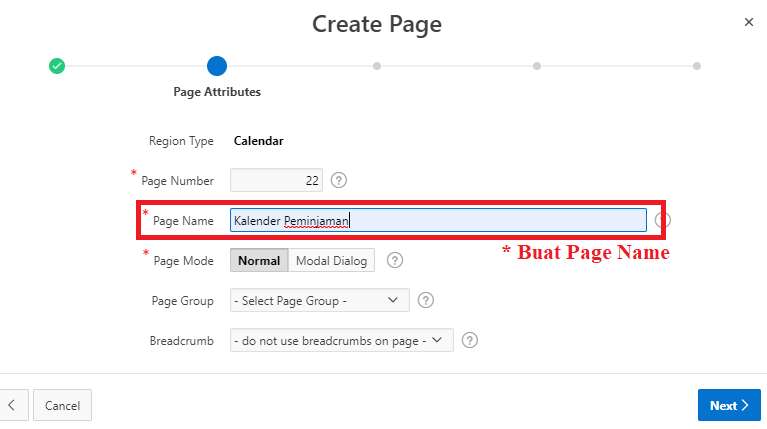
\includegraphics[scale=0.4]{figures/date/date2.png}
        \caption{\textit{Membuat Page Name Calendar}}
        \label{Membuat Page Name Calendar}
    \end{figure}
    \item[3]Membuat Menu Navigasi, ikuti intruksi warna, lihat pada Gambar 9.10.
    \begin{figure}
        \centering
        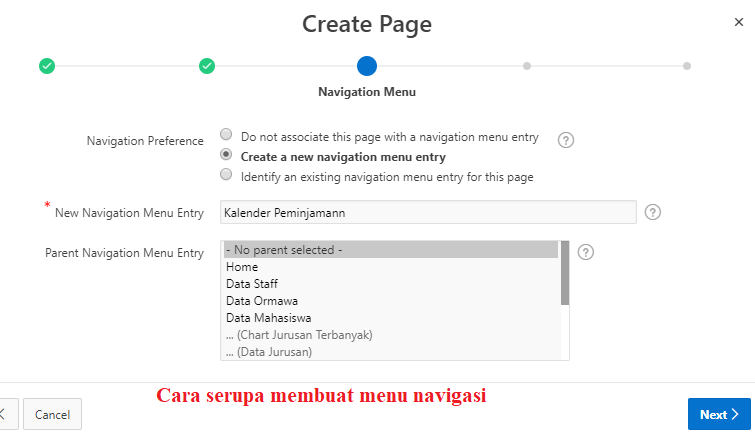
\includegraphics[scale=0.4]{figures/date/date3.png}
        \caption{\textit{Membuat Menu Navigasi Calendar}}
        \label{Membuat Menu Navigasi Calendar}
    \end{figure}
    \item[4]Memilih tabel, ikuti intruksi warna, lihat pada Gambar 9.11.
    \begin{figure}
        \centering
        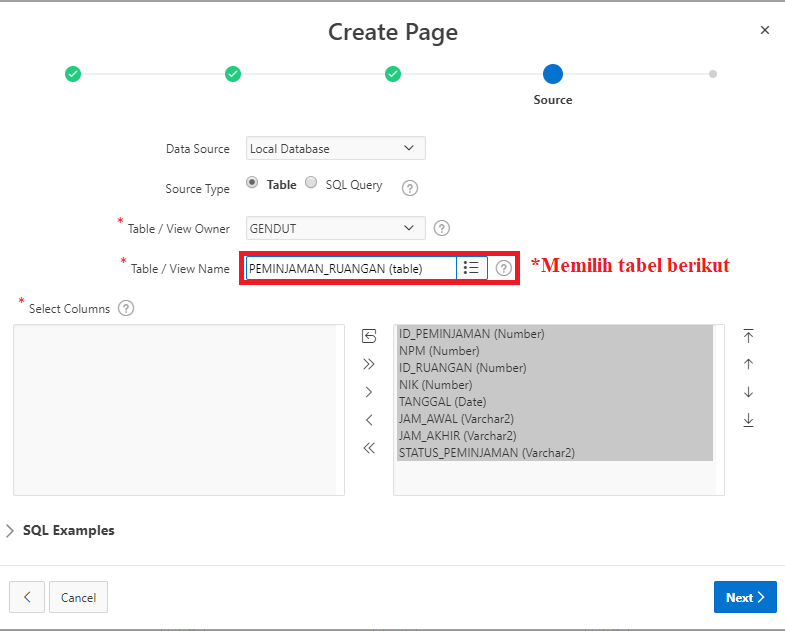
\includegraphics[scale=0.4]{figures/date/date4.png}
        \caption{\textit{Memilih Tabel Calendar}}
        \label{Memilih Tabel Calendar}
    \end{figure}
    \item[5]Membuat settingan tanggal yang akan ditampilkan, ikuti intruksi warna, lihat pada Gambar 9.12.
    \begin{figure}
        \centering
        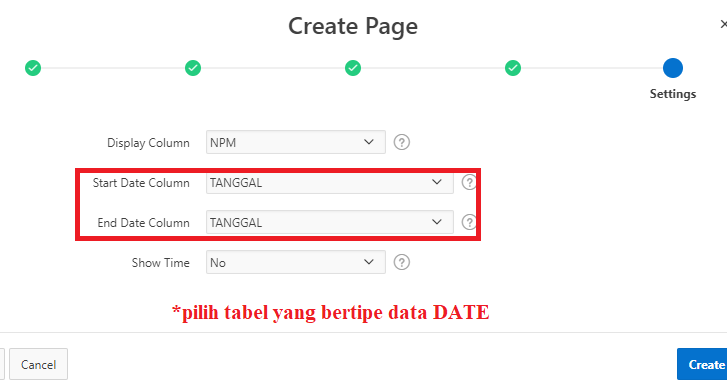
\includegraphics[scale=0.4]{figures/date/date5.png}
        \caption{\textit{Membuat Settingan Calendar}}
        \label{Membuat Settingan Calendar}
    \end{figure}
    \item[6]Anda bisa langsung cek dengan RUN aplikasi anda, lihat pada Gambar 9.13.
    \begin{figure}
        \centering
        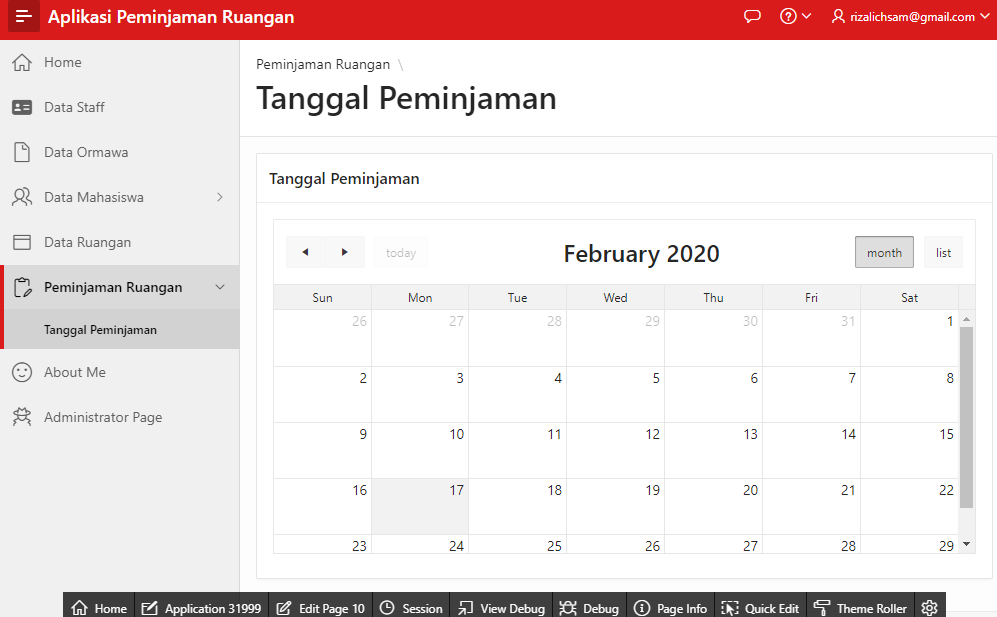
\includegraphics[scale=0.4]{figures/date/date6.png}
        \caption{\textit{Tampilan CALENDAR}}
        \label{Tampilan Calendar}
    \end{figure}
\end{itemize}